\chapter{Theory} 
\label{ch:theory}

\minitoc

%What's the standard model all about? 

%\section{In the beginning...}
%\section{Some other stuff}



%\section{The Standard model of Particle of Physics}
\section{The weak force in \bquark-hadron decays}

Ground state \bquark-hadrons can only decay weakly as the \bquark must change flavour to one of the first or second generation quarks.
These decays were first observed ... with lifetime ...
Although the weak interaction dictates the core of the process, the contributions from the strong force are unavoidable. In the SM quarks abide by \emph{confinement}, preventing bare quarks from propagating unhindered. Instead quarks are only ever observed in bound states, or hadrons, with other quarks or anti-quarks. Therefore the observation of the weakly decaying \bquark-quark is necessarily accompanied by the strong interaction governing the harmonisation of the initial and final state quarks.


\subsection{The weak force}

The weak and electromagnetic forces are unified in the SM through the gauge group $\text{SU}(2)\times\text{U}(1)$.

{\color{Red}
\begin{itemize}
\item Photon and Z mix
\item Hyper charge
\item couplings
\item Parity in the weak force
\item CP? 
\end{itemize}}

\subsection{Weak interactions of quarks}

{\color{Red}
\begin{itemize}
\item semileptonic decays 
\item cabibbo formulated angle
\item  
\end{itemize}}


\subsection{The CKM matrix}

{\color{Red}
\begin{itemize}
\item introduce idea of CP violation
\item Observation of CP violation? 
\end{itemize}}

\subsection{\bquark-hadron physics}
The b stands for beauty
{\color{Red}
\begin{itemize}
\item CP violation in the B sector
\item \B meson mixing
\item lifetime maybe? 
\end{itemize}}

\subsection{QCD and hadronisation}
{\color{Red}
\begin{itemize}
\item Explain why predictions are hard
\item lattice QCD
\item light cone sum rules? 
\end{itemize}}

\section{Annihilation topology decays}

{\color{Red}
\begin{itemize}
\item Talk about \D and other annihilation topologies 
\item Find origin of hadronic uncertainties 
\end{itemize}}


\subsection{Pure annihilation topology decays}
{\color{Red}
\begin{itemize}
\item Pure annihilation - charmless Bc
\end{itemize}}
\subsection{Other annihilation decays}

{\color{Red}
\begin{itemize}
\item non pure - donals Bc 
\end{itemize}}

\section{Rescattering}

{\color{Red}
\begin{itemize}
\item What is rescattering?
\item Examples of it?
\item Why it's expected to be small
\end{itemize}}

\section{Theoretical predictions for the \decay{\Bp}{\Dsp\phiz} decay}

%%%%%%%%%%%%%%%%%%%%%%%%%%%%%%%%%%%%%%%%%%%%%%%%%%%%%%%%%%
\begin{figure}[!h]
    \centering
    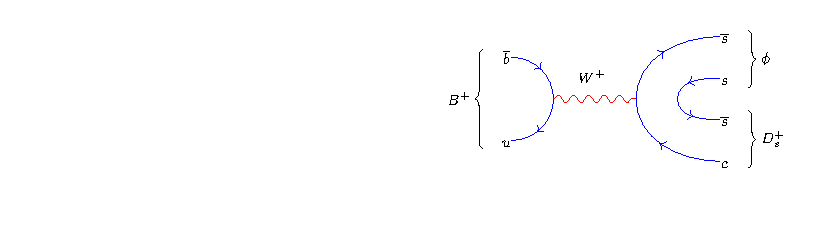
\includegraphics[width=0.6\textwidth]{figs/Theory/B2DsPhi.pdf}
    \caption{\decay{\Bp}{\Dsp\phiz} }
    \label{fig:Theory_DsPhiDiagram}   
\end{figure}
%%%%%%%%%%%%%%%%%%%%%%%%%%%%%%%%%%%%%%%%%%%%%%%%%%%%%%%%%%



{\color{Blue}
In the SM, the decay $\decay{\Bp}{\Dsp\phi}$ proceeds dominantly via the annihilation diagram shown in Fig.~\ref{fig:Theory_DsPhiDiagram}. 
This suppressed topology requires the wave functions of the incoming quarks to overlap sufficiently to annihilate into a virtual \Wp boson. 
The decay is further suppressed by the small magnitude of the CKM matrix element \Vub associated with the annihilation vertex. 


}

\subsection{Standard model predictions}
{\color{Blue}
Several SM predictions have been made for the branching fraction of the $\decay{\Bp}{\Dsp\phi}$ decay~\cite{Zou:2009zza, Mohanta:2002wf, Mohanta:2007uu, Lu:2001yz}, using input from lattice calculations~\cite{fB:2013HPQCD,fB:2016ETM, fB:2016Fermi}. These predictions are in the range $(1-7)\times10^{-7}$, where the limit on the precision is dominated by hadronic uncertainties. 

In addition, unlike many rare hadronic decays including $\decay{\Bp}{\Dsp\Kp\Km}$, possible contributions from rescattering effects are expected to be small, for example contributions from intermediate states such as $\decay{\Bp}{\Dsp\omega}$~\cite{Gronau:2012gs}.

}

{\color{Red}
\begin{itemize}
\item Find origin of hadronic uncertainties 
\end{itemize}}

\subsection{BSM models and predictions}
{\color{Blue}
However, additional diagrams contributing to this decay can arise in some extensions of the SM, such as supersymmetric models with R-parity 
violation. They could enhance the branching fraction and/or produce large \CP asymmetries~\cite{Mohanta:2002wf, Mohanta:2007uu}, which makes the $\decay{\Bp}{\Dsp\phi}$ decay a promising place to search for new physics beyond the SM.\footnote{Charge conjugation is implied throughout this paper. Furthermore, $\phi$ denotes the $\phi(1020)$ resonance.}
}

{\color{Red}
\begin{itemize}
\item Higgs doublet
\item SUSY 
\item include feynman diagrams
\item small intro into models
\end{itemize}}

\subsection{Previous measurements}

{\color{Blue}
The \lhcb experiment reported evidence for the decay $\decay{\Bp}{\Dsp\phi}$ using $pp$ collision data corresponding to an integrated luminosity of 1\invfb taken during 2011, at a centre-of-mass energy of 7\tev~\cite{Aaij:2012zh}. A total of $6.7^{+4.5}_{-2.6}$ candidates was observed. The branching fraction was determined to be 

\begin{equation}
\mathcal{B}(\decay{\Bp}{\Dsp\phi}) = (1.87^{+1.25}_{-0.73} \pm 0.19 \pm 0.32) \times 10^{-6},
\end{equation}
where the first uncertainty is statistical, the second is systematic and the third is due to the uncertainty on the branching fraction of the decay $\decay{\Bp}{\Dsp\Dzb}$, which was used as normalisation. 
Given the large uncertainties on both the theoretical and experimental values, the previously measured value is consistent with the range of SM values given above.
}

{\color{Red}
\begin{itemize}
\item Include plot and measurement
\item say something about similarites 
\end{itemize}}


\section{Theoretical predictions for the \decay{\Bp}{\Dsp\Kp\Km} decay}


%%%%%%%%%%%%%%%%%%%%%%%%%%%%%%%%%%%%%%%%%%%%%%%%%%%%%%%%%%
\begin{figure}[!h]
    \centering
    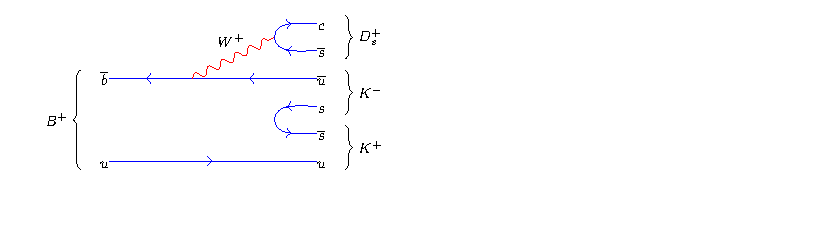
\includegraphics[width=0.6\textwidth]{figs/Theory/B2DsKK.pdf}
    \caption{\decay{\Bp}{\Dsp\Kp\Km} }
    \label{fig:Theory_DsKKDiagram}   
\end{figure}
%%%%%%%%%%%%%%%%%%%%%%%%%%%%%%%%%%%%%%%%%%%%%%%%%%%%%%%%%%



{\color{Blue}
The decay $\decay{\Bp}{\Dsp\Kp\Km}$ is mediated by a $\decay{\bquarkbar}{\uquarkbar}$ transition shown in Fig.~\ref{fig:Theory_DsKKDiagram} and is therefore suppressed in the Standard Model (SM) due to the small size of the Cabibbo-Kobayashi-Maskawa (CKM) matrix element \Vub. 
}


{\color{Red}
\begin{itemize}
\item explain what a dalitz plot is
\end{itemize}
}

\subsection{Standard model predictions}
{\color{Blue}
The branching fraction for this decay is currently not measured, however a similar decay, \decay{\Bp}{\Dsp \piz}, has been observed with a branching fraction of $\mathcal{B}(\decay{\Bp}{\Dsp \piz}) = (1.5 \pm 0.5) \times 10^{-5}$~\cite{Aubert:2006xy}.
}


{\color{Red}
\begin{itemize}
\item talk about \decay{\Bp}{\Dsp\piz}
\item Could talk about \decay{\Bp}{\Dp\Kp\pim} and estimate   
\end{itemize}}

\subsection{Previous measurements}



